To validate the importance of the balance between robustness and flexibility in the CPG circuits, as provided by cycle-by-cycle dynamical invariants present in its dynamics discussed in this chapter, we include in this section a first approach of the translation of dynamical invariants into an effective motor locomotion in a Functional-Living-Circuit-Hybrot (FLC-Hybrot). This work was published in \cite{amaducci_hybrid_2020,amaducci_controlling_2021}. In this first step into the applications in robotics of the variability time contrains found in CPGs, we built an hexapod robot whose legs performed oscillatory motions to move forward. The period and amplitude of these oscillations were determined by the sequential cycle-by-cycle activity of the CPG neurons recorded from the living preparation and sent online to the robot. At the same time, the hybrot included a light sensor and sent feedback information regarding the light conditions around it back to the neural circuit in the form of an electrical current. These stimuli modified the behavior of the cells, resulting in a change of the hybrot locomotion, preserving always the required motor coordination, and therefore forming a real-time closed-loop interaction among living and electronic components (Figure \ref{fig:robot_results_summary} shows a summary of these interactions). The goal of the FLC-Hybrot is to demonstrate that a dynamical principle of the functional living circuit can be used to coordinate the locomotion with sensory feedback from the robot. In our case, we use the presence of dynamical invariants in the form of robust relationships between the time intervals that build the cycle-by-cycle activity of the CPG in the neurons of the pyloric CPG in \textit{Carcinus maenas}, which are sustained under any circumstances even when there are external inputs to the circuit, to modulate the behavior of the robot. There is a detailed description of the experimental setup of the robot in section \ref{sec:robot setup}

\begin{figure}[hbt!]
	\begin{center}
		% \includegraphics[width=\linewidth]{images/robot/robot_results_summary}
		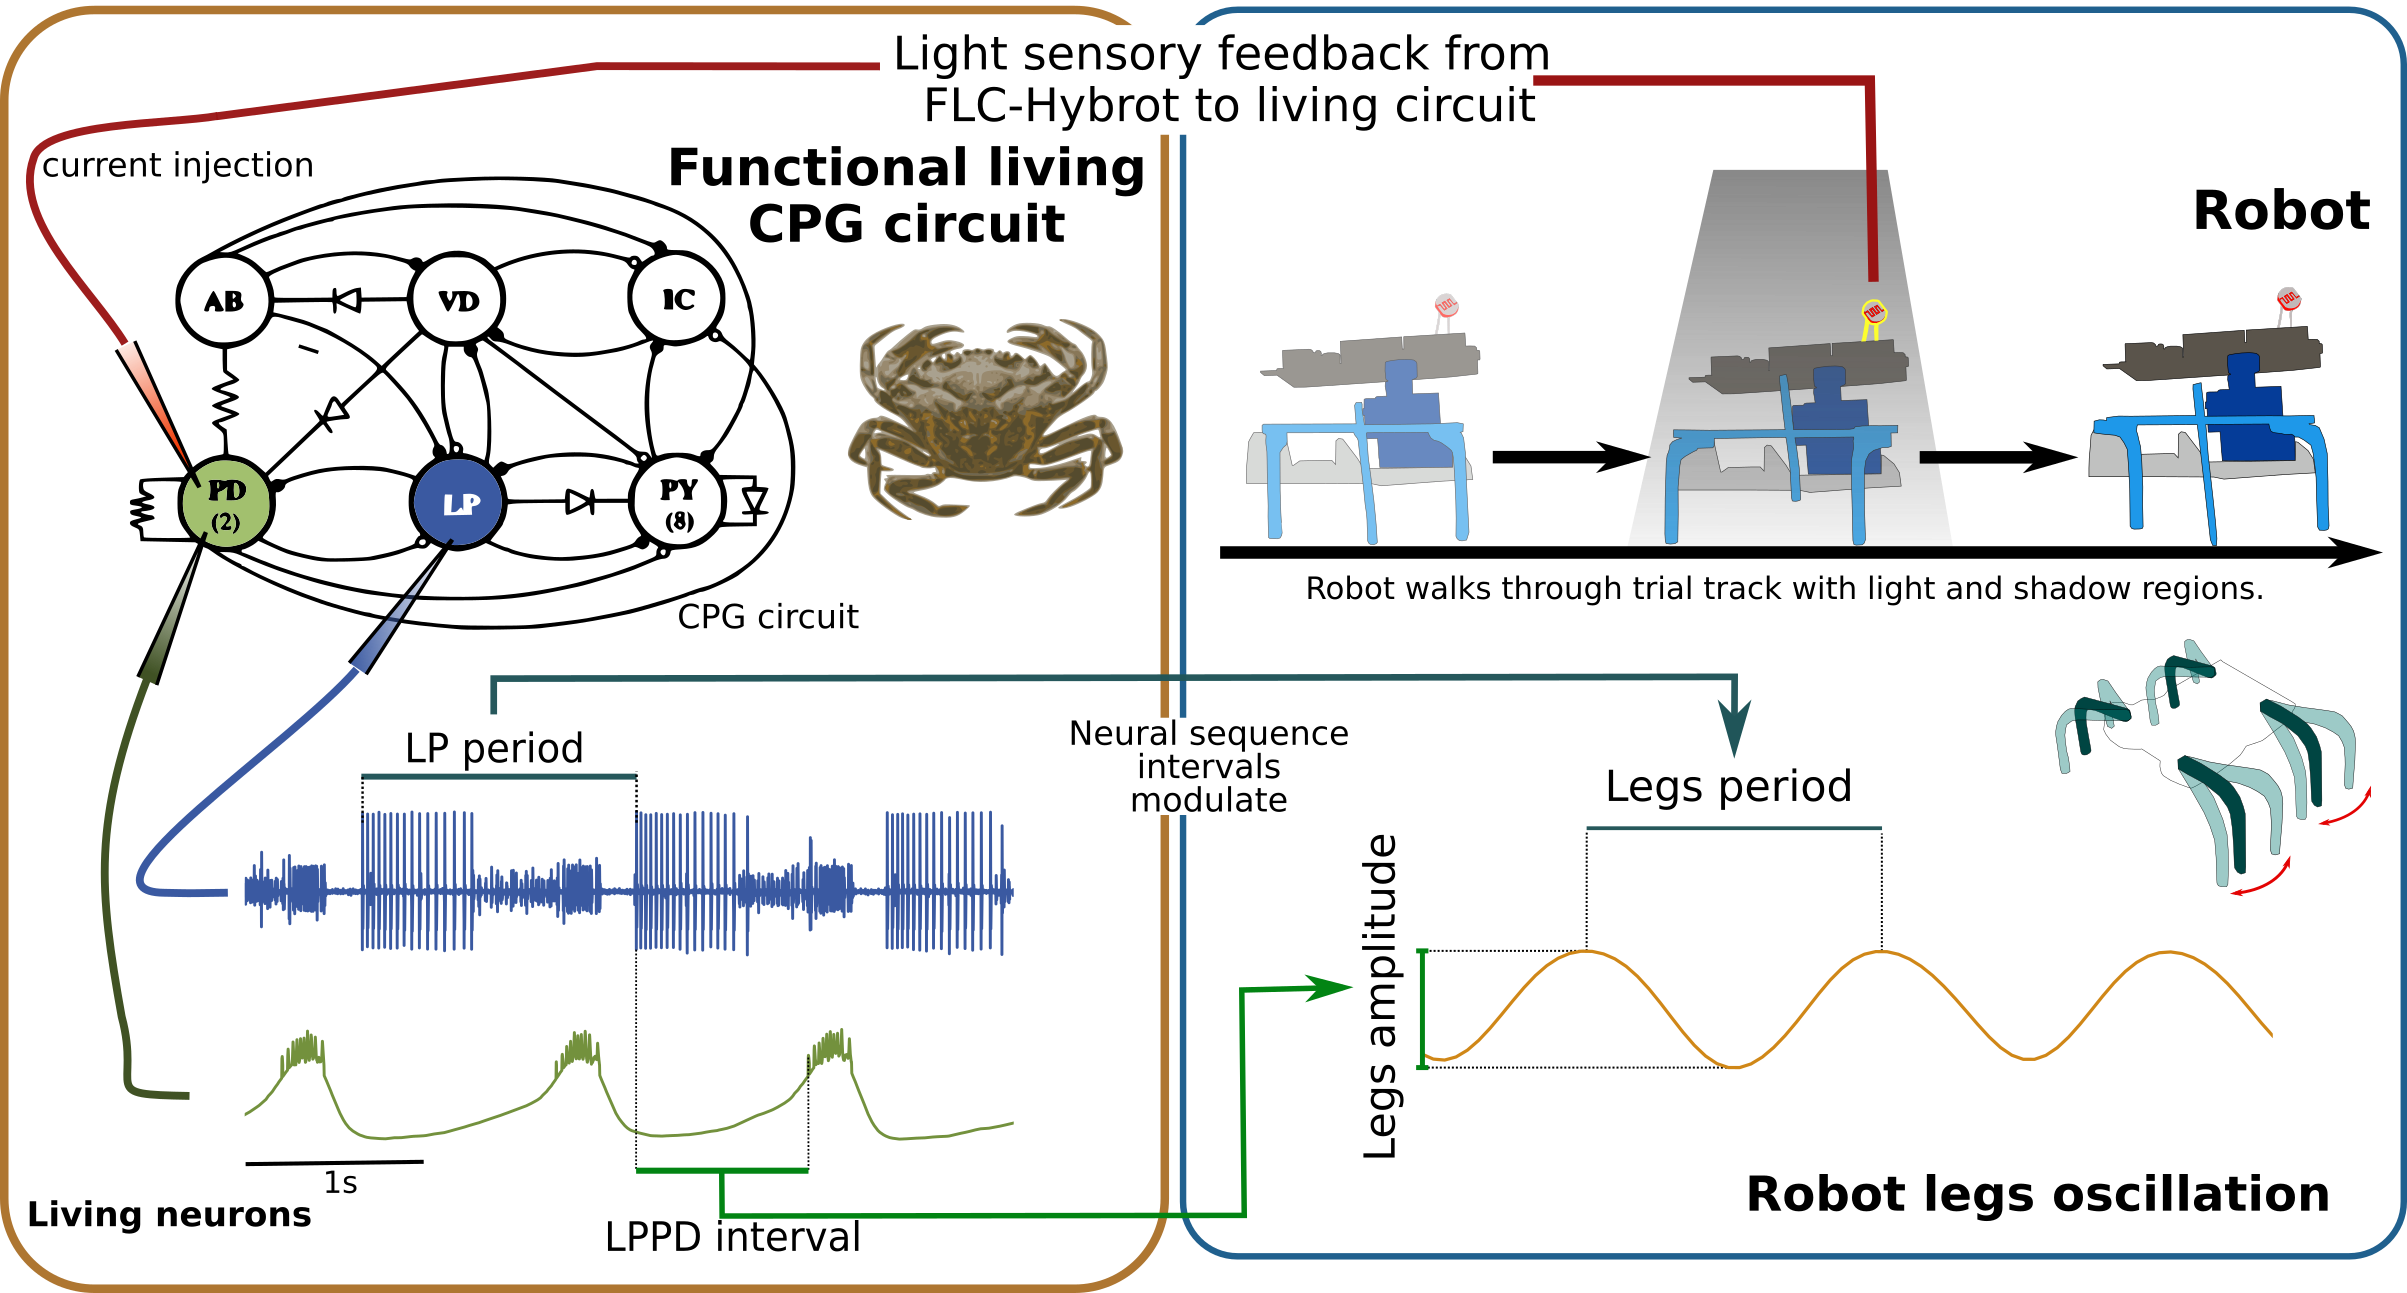
\includegraphics[width=\textwidth]{img/invariants/robot/Figure1_experiment_design_v1.png}
	\end{center}
	\caption{Representation of the FLC-Hybrot paradigm design. Neural dynamics from a functional living CPG circuit are recorded online and used to coordinate the robot movement in real-time. Activity from the PD neuron is recorded intracellularly (green trace), while the LP bursts are extracted from the nerve's extracellular signal (blue trace). This robot walks through a trial track with interspersed light and shadow regions. When the robot's light sensor detects that it is located under a shadow, it sends feedback current to the living circuit. CPG dynamics change as a reaction to the injected current, thus modifying the robotic locomotion. The following video shows an example of this experiment \url{https://youtu.be/ny2dJGbG8lo}.}
	\label{fig:robot_results_summary}
\end{figure}


To validate the adequate locomotion of the FLC-Hybrot when modulated by the pyloric CPG online behavior, as well as the living circuit real-time adaptation to the injected feedback, we performed a set of experiments employing a 1.5 meters long trial track. Along this surface there were interspersed segments of lights and shadows. This configuration caused the FLC-Hybrot to alter its behavior several times during the experiment due to the injection of current into the PD neuron when it walked under a shadow. The current injected in the cell in a shadow section varied from one experiment to another, according to the neurons response to the stimuli. No current was injected when the robot was located on a luminous area. The following video illustrates one of such experiments \url{https://youtu.be/Dltec7TeGso}.

\begin{figure}[hbt!]
	\begin{center}
		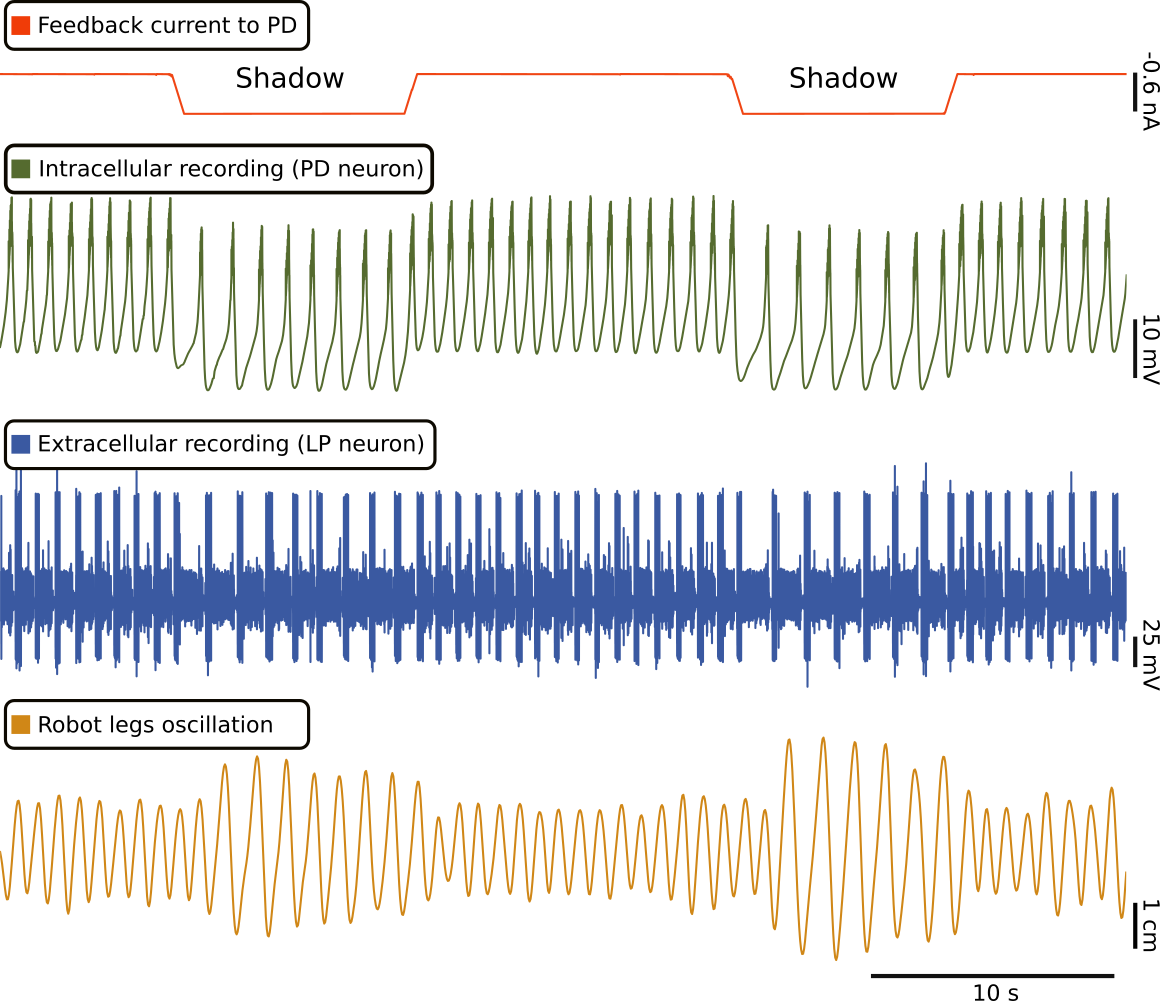
\includegraphics[width=0.8\linewidth]{./img/invariants/robot/robot_results_validation}
	\end{center}
	\caption{Flexible hybrot adaptation to environmental changes when noticed by the robot sensors and associated coordinated locomotion. When the robot entered a shadow section, it sent sensory feedback to the living CPG in the form of positive electrical current (red trace). Blue and green traces are recordings of the extracellular and intracellular (PD neuron) activity of the circuit and display the change caused by the feedback current injection in the PD neuron, slowing down the CPG rhythm. The oscillatory movement of the robot legs is represented in the brown trace and it can observed that a variation in the CPG rhythm leads to a change in the robotic locomotion, modifying both the period and the amplitude of the oscillation. 
		%This effect can be seen more clearly in the bottom panel, where both the LP neuron instantaneous bursting period (blue) and the robot legs oscillation period (brown) are plotted together, showing how the latter is modulated by the former.
	}
	\label{fig:robot_results_validation}
\end{figure}

Figure \ref{fig:robot_results_validation} shows the results for one of these tests. We observe an alteration of the neural when -0.6nA current is inserted into the circuit, causing its rhythm to slow down while also modifying the PD neuron membrane's potential amplitude. This change is immediately reversed as soon as the current goes back to zero, restoring its previous behavior. Concerning the robot's locomotion, a variation in the legs' oscillation is observed just after the neurons alter their functioning. Despite the successive changes in the amplitude and period of its legs' oscillation, the FLC-Hybrot maintained a coordinated and effective locomotion during the whole experiment. 

We know that in the pyloric CPG there is a sequential dynamical invariant, in the form of a linear relation between the LP neuron period and the LPPD interval. These are the intervals used to modulate the amplitude and period of the legs oscilation in the robot. This constrain was effectively transferred to the robot locomotion. Figure \ref{fig:robot_results_invariant} shows a comparison between the living CPG and the robot dynamical invariant, with the later reaching an $R^2$ correlation of 0.87 despite the lack of precision of its servomotors. It displayed the same correlation between its legs oscillation period and amplitude, which were modulated by the two previous temporal intervals.

\begin{figure}[hbt!]
	\begin{center}
		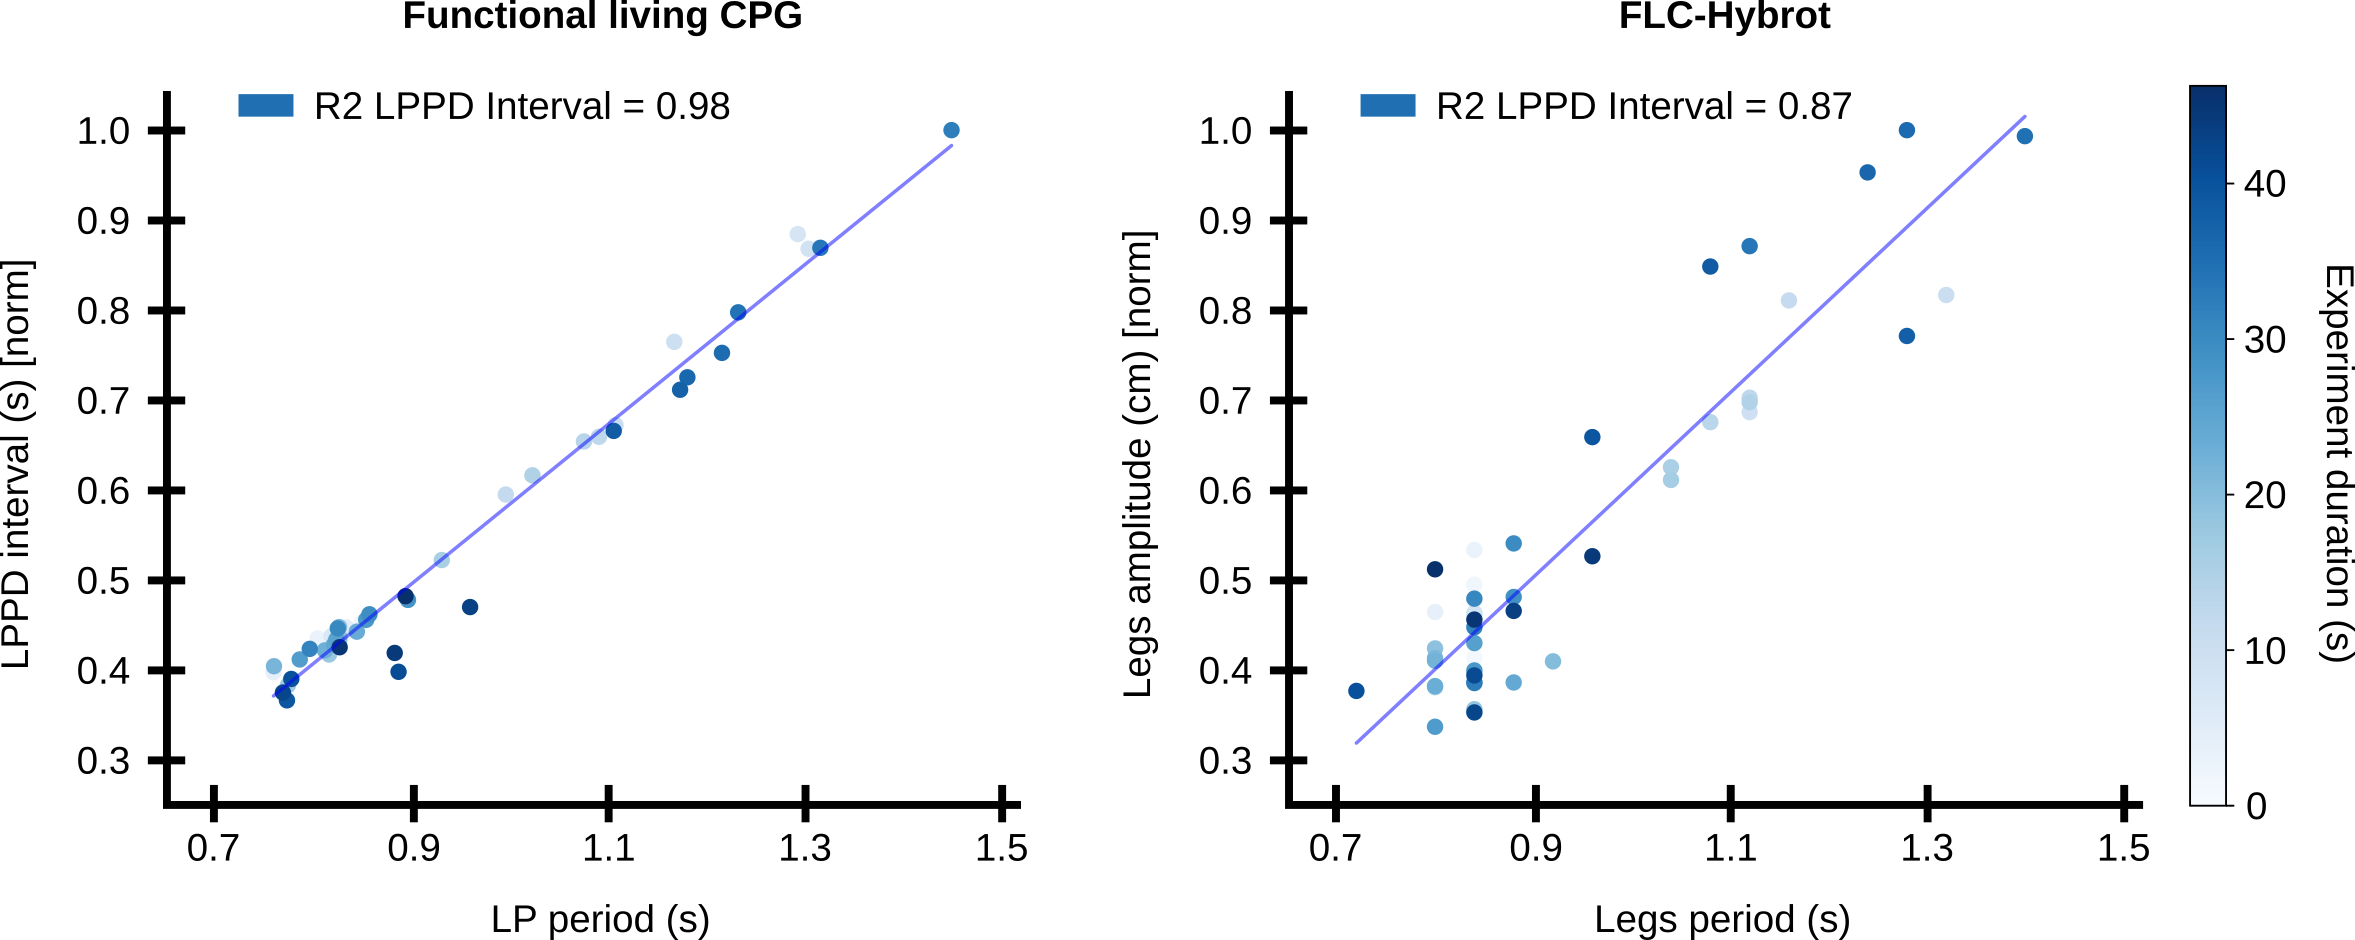
\includegraphics[width=\linewidth]{./img/invariants/robot/robot_results_invariant}
	\end{center}
	\caption{\textbf{Left:} dynamical invariant present in the living CPG activity during the validation test, represented as a linear relation between the LP neuron bursting period and the LPPD interval cycle-by-cycle. \textbf{Right:} dynamical invariant present in the FLC-Hybrot locomotion during the validation test, represented as a linear relation between its legs oscillation period and amplitude cycle-by-cycle. The dynamical invariant property is effectively translated from the living CPG to the robot locomotion, codified as: Robot period = LP period, Robot amplitude = LPPD interval * factor.}
	\label{fig:robot_results_invariant}
\end{figure}

This tested scenario, can help simulate context change situations in which the CPG rhythm is alterated and there is a change of variability reflected in the relations between the intervals cycle-by-cycle. The reproduction of biological dynamics with its time constraints can have strong implications in robotics locomotion but also in neurorehabilitation processes. It can also help explain and associated the observed phenomena of sequential dynamical invariants to its living functionality.
